% -*- LaTeX -*-
% -*- coding: utf-8 -*-
%
% michael a.g. aïvázis <michael.aivazis@para-sim.com>
% (c) 2003-2017 all rights reserved
%

\section{applications}

% --------------------------------------
\subsection{shells}
\begin{frame}
%
  \label{frame:pyre-plexus}
%
  \frametitle{The \component{Plexus} structure}
%
  \vskip -3ex
  \only<1>{
\includegraphics[height=0.9\textheight]{pyre-plexus-base}}
  \only<2>{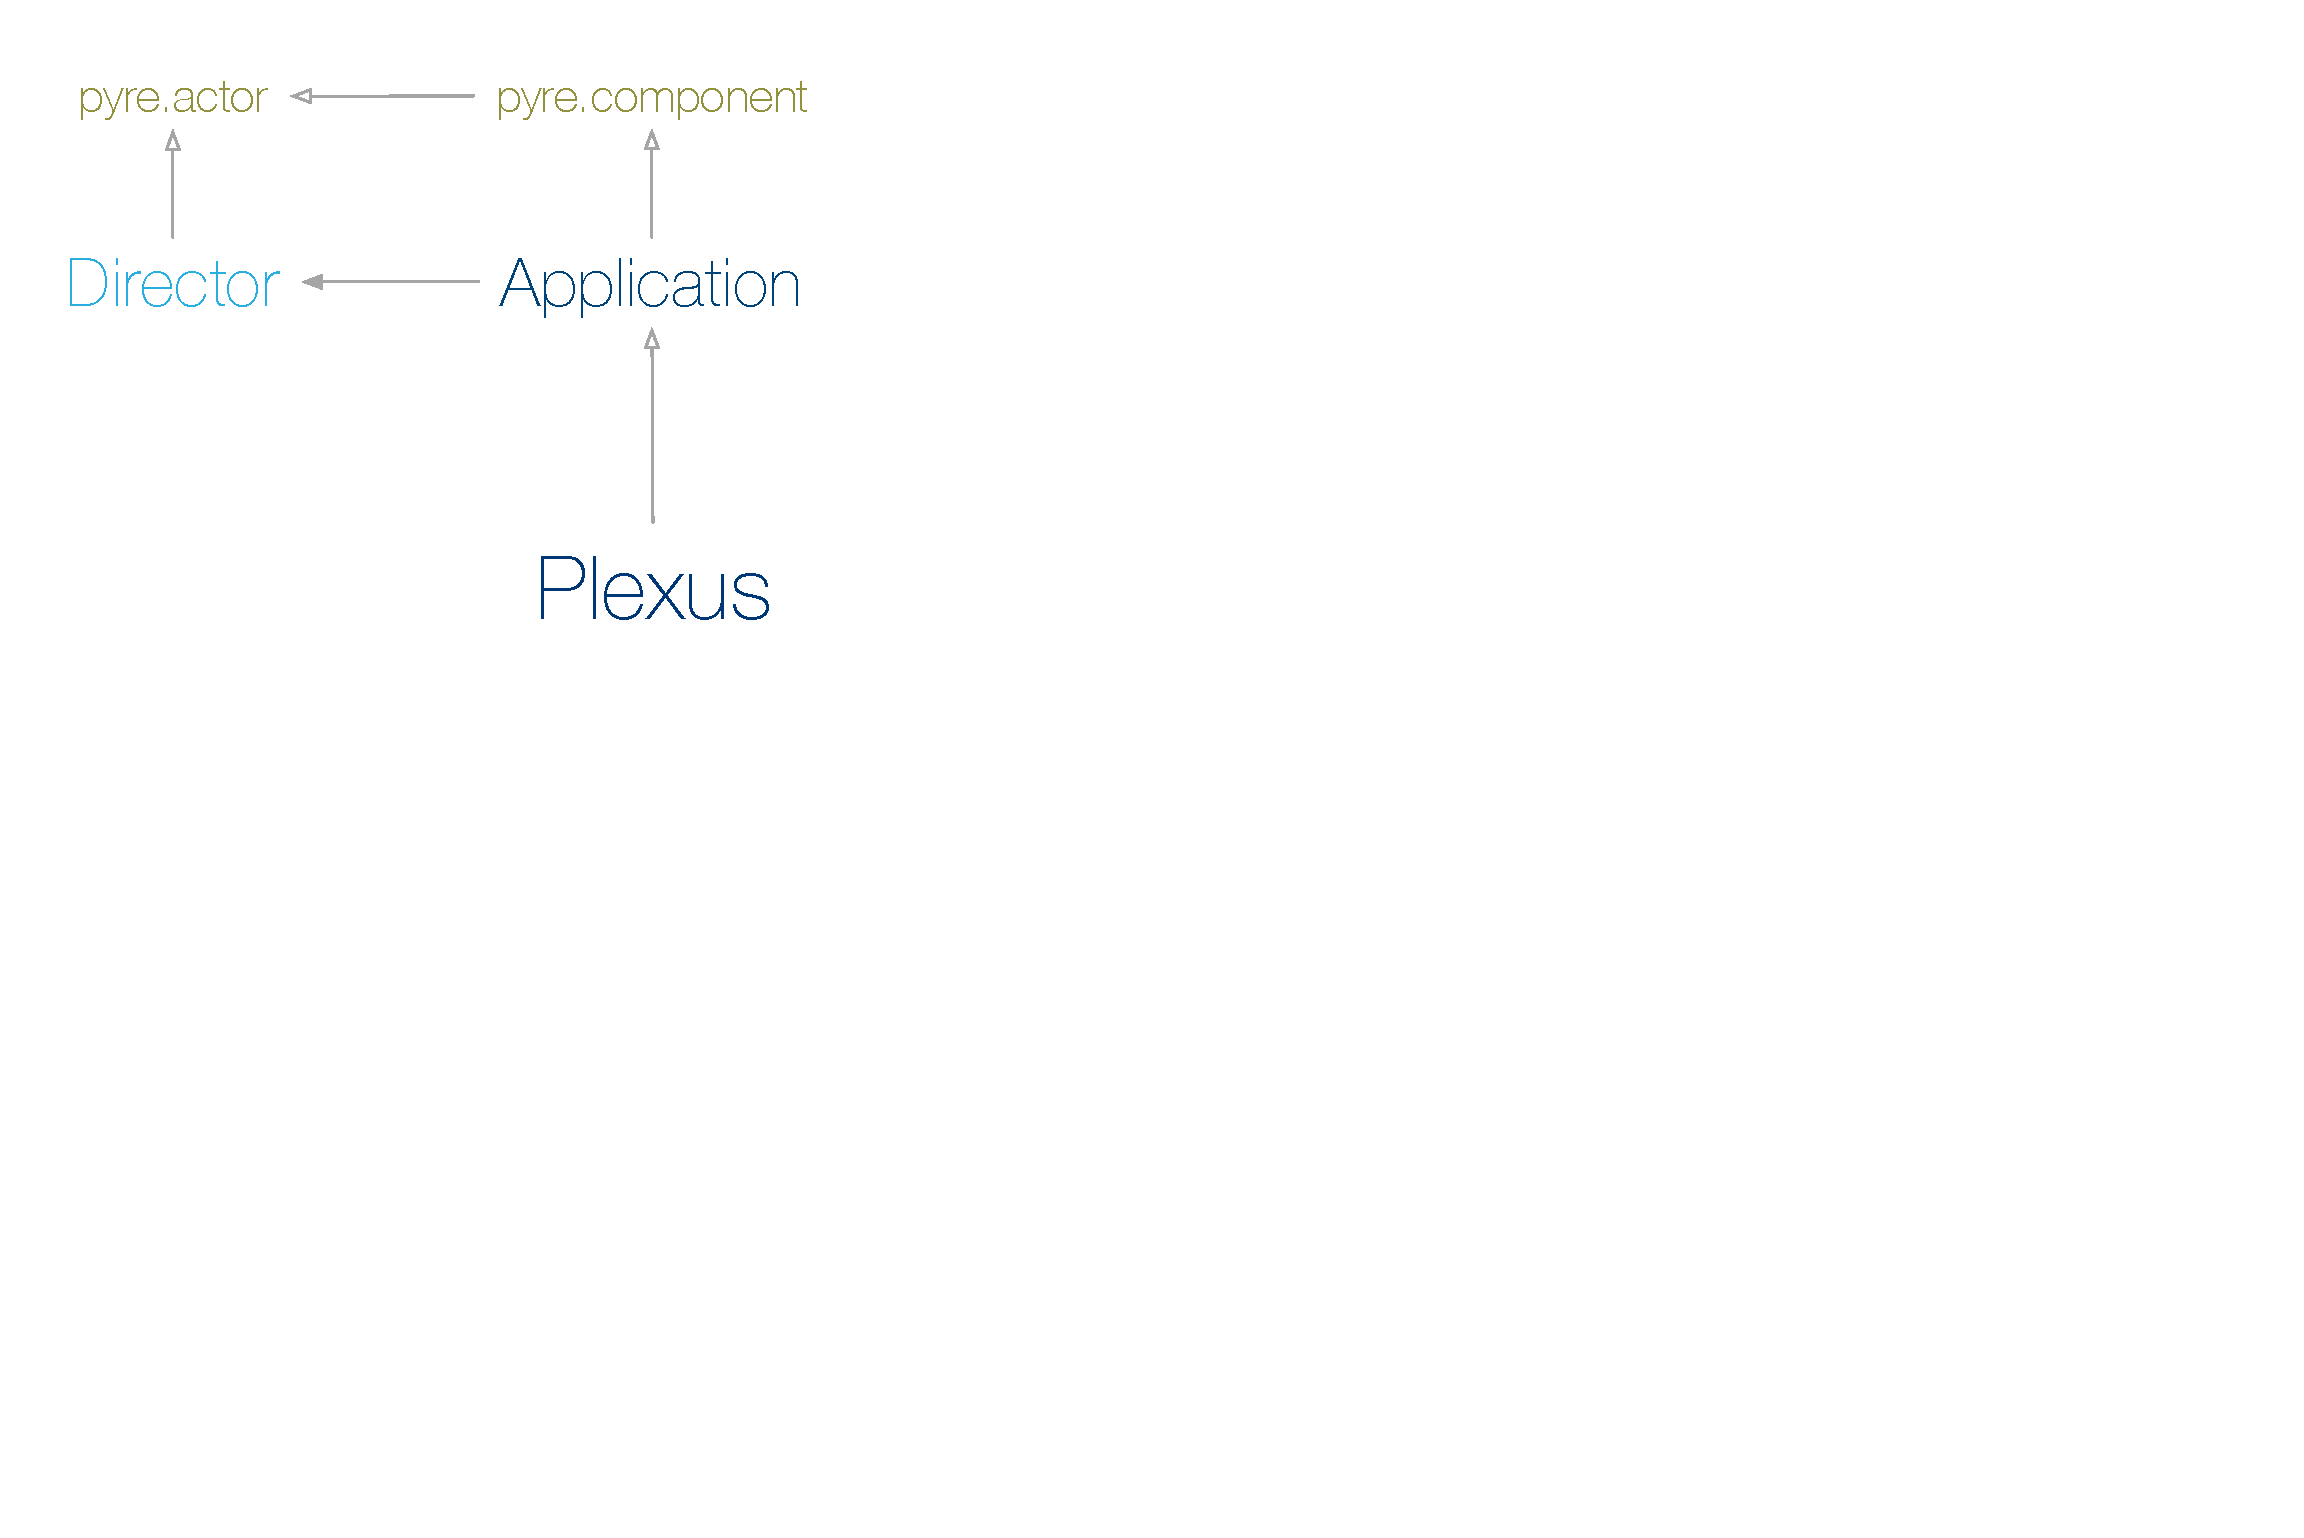
\includegraphics[height=0.9\textheight]{pyre-plexus-pedigree}}
  \only<3>{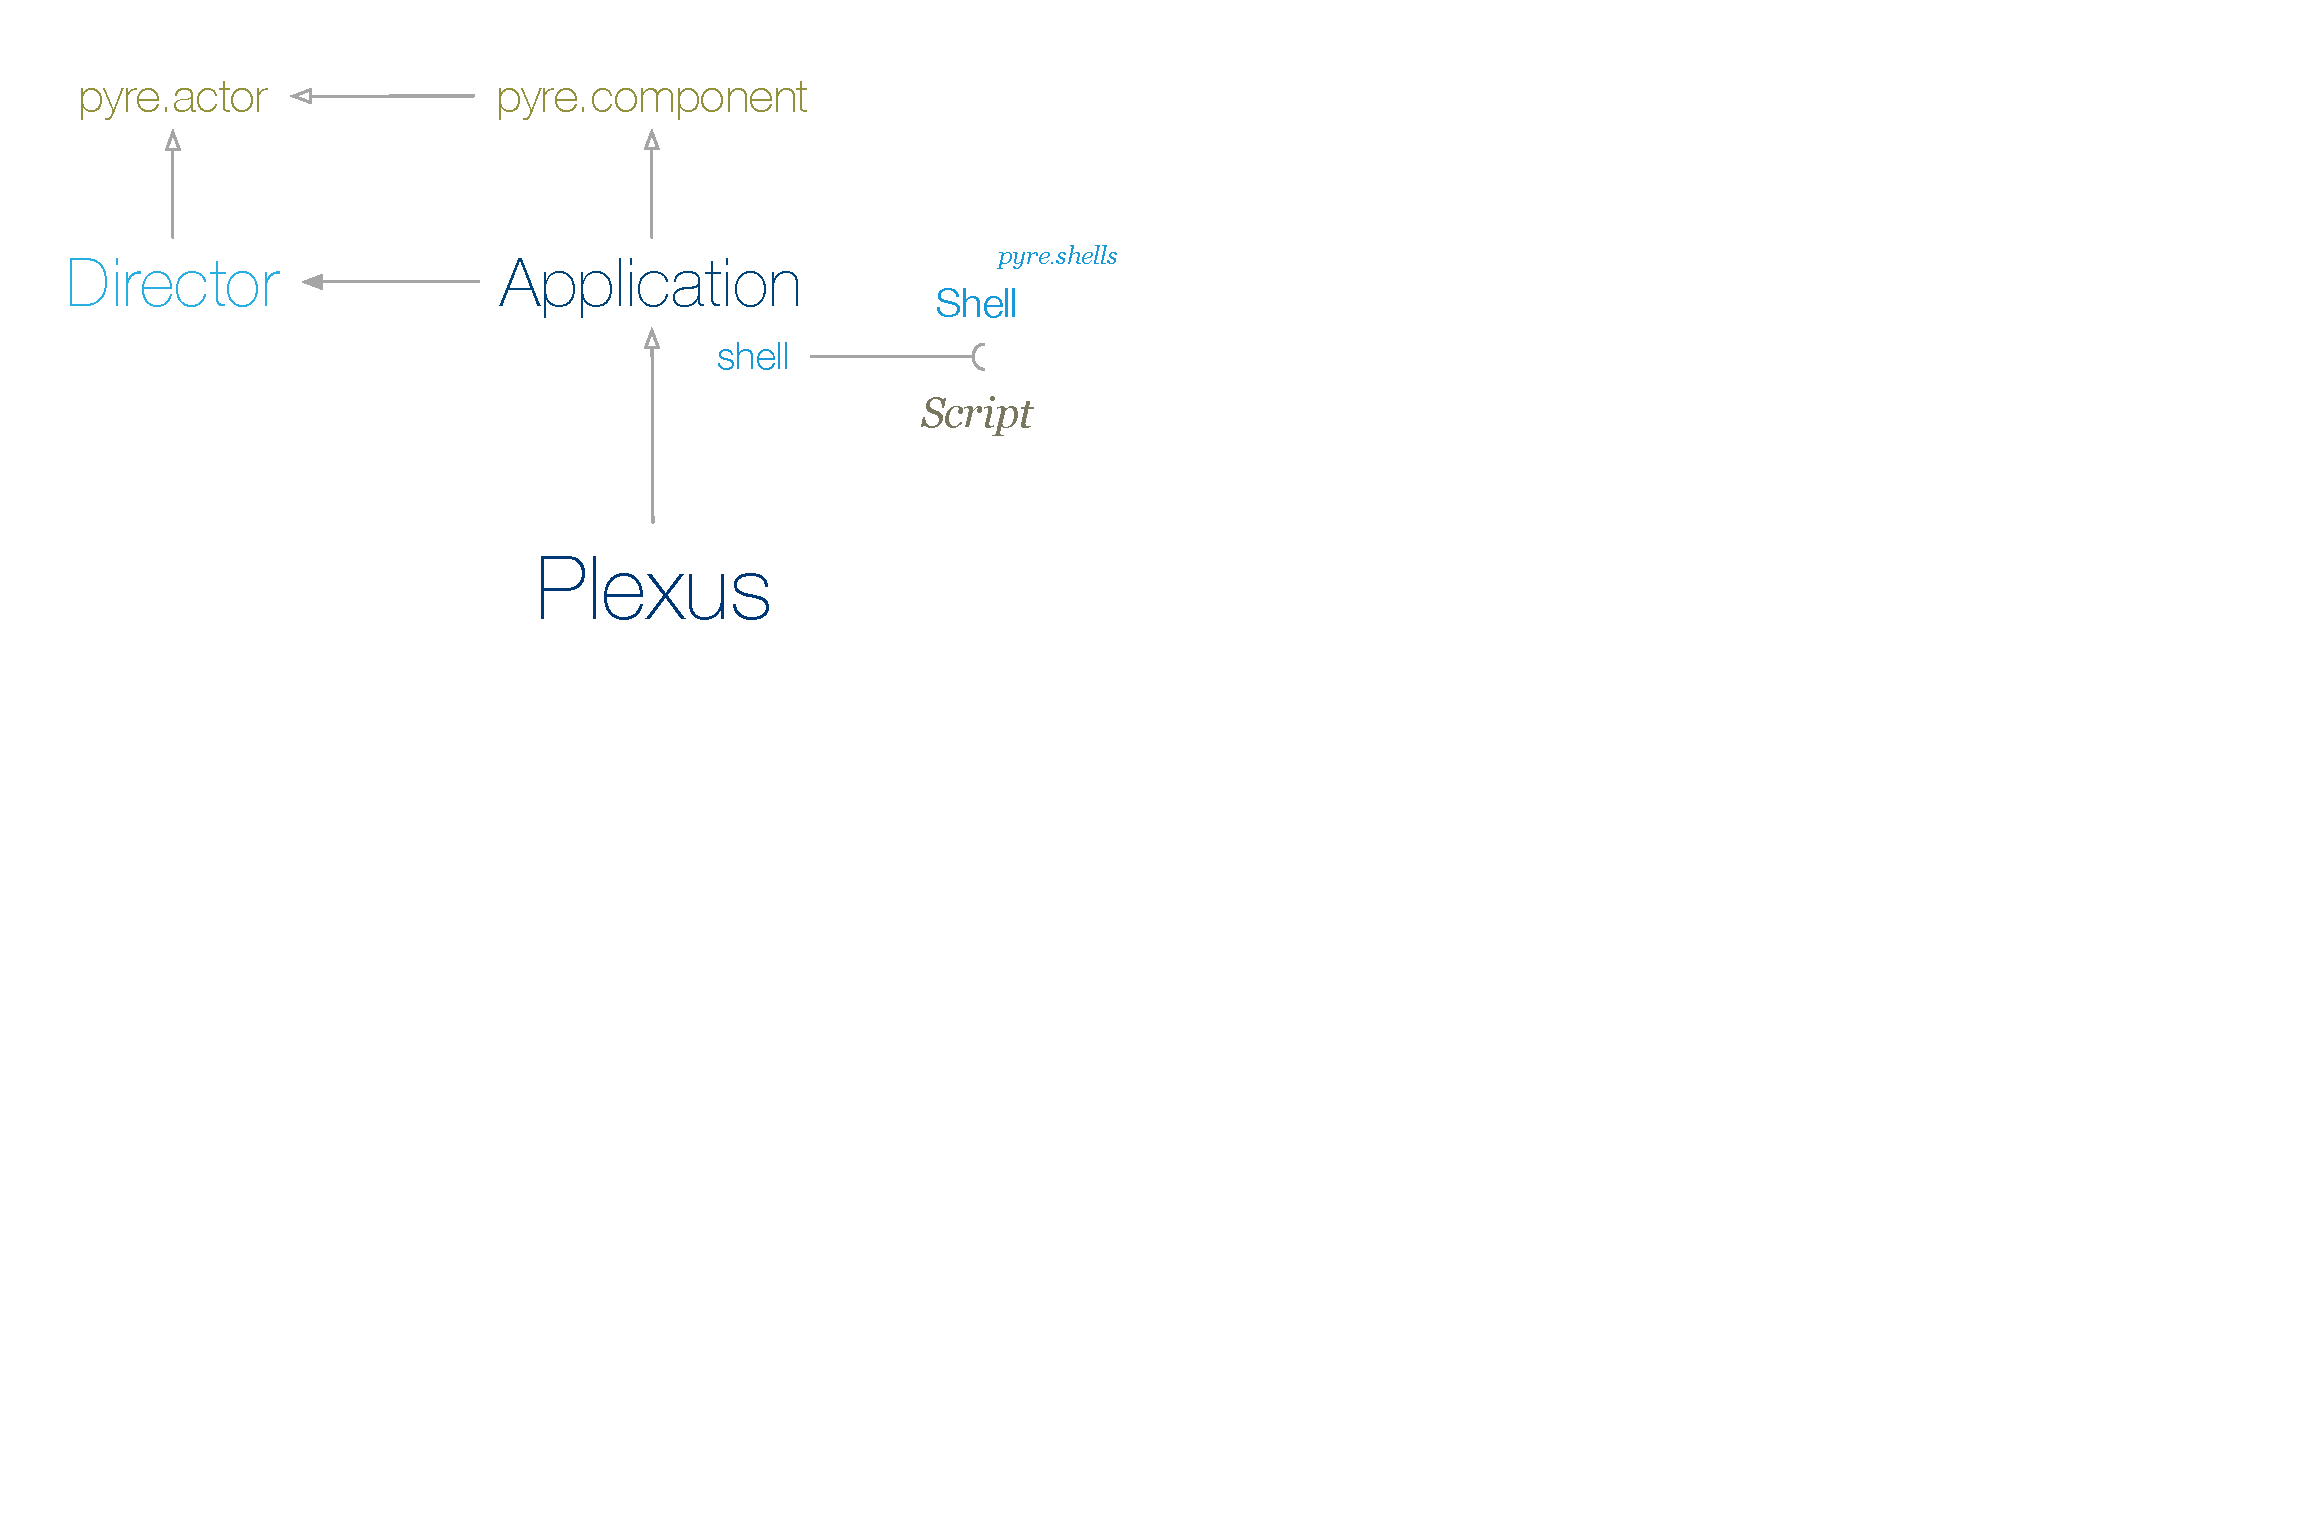
\includegraphics[height=0.9\textheight]{pyre-plexus-traits}}
  \only<4>{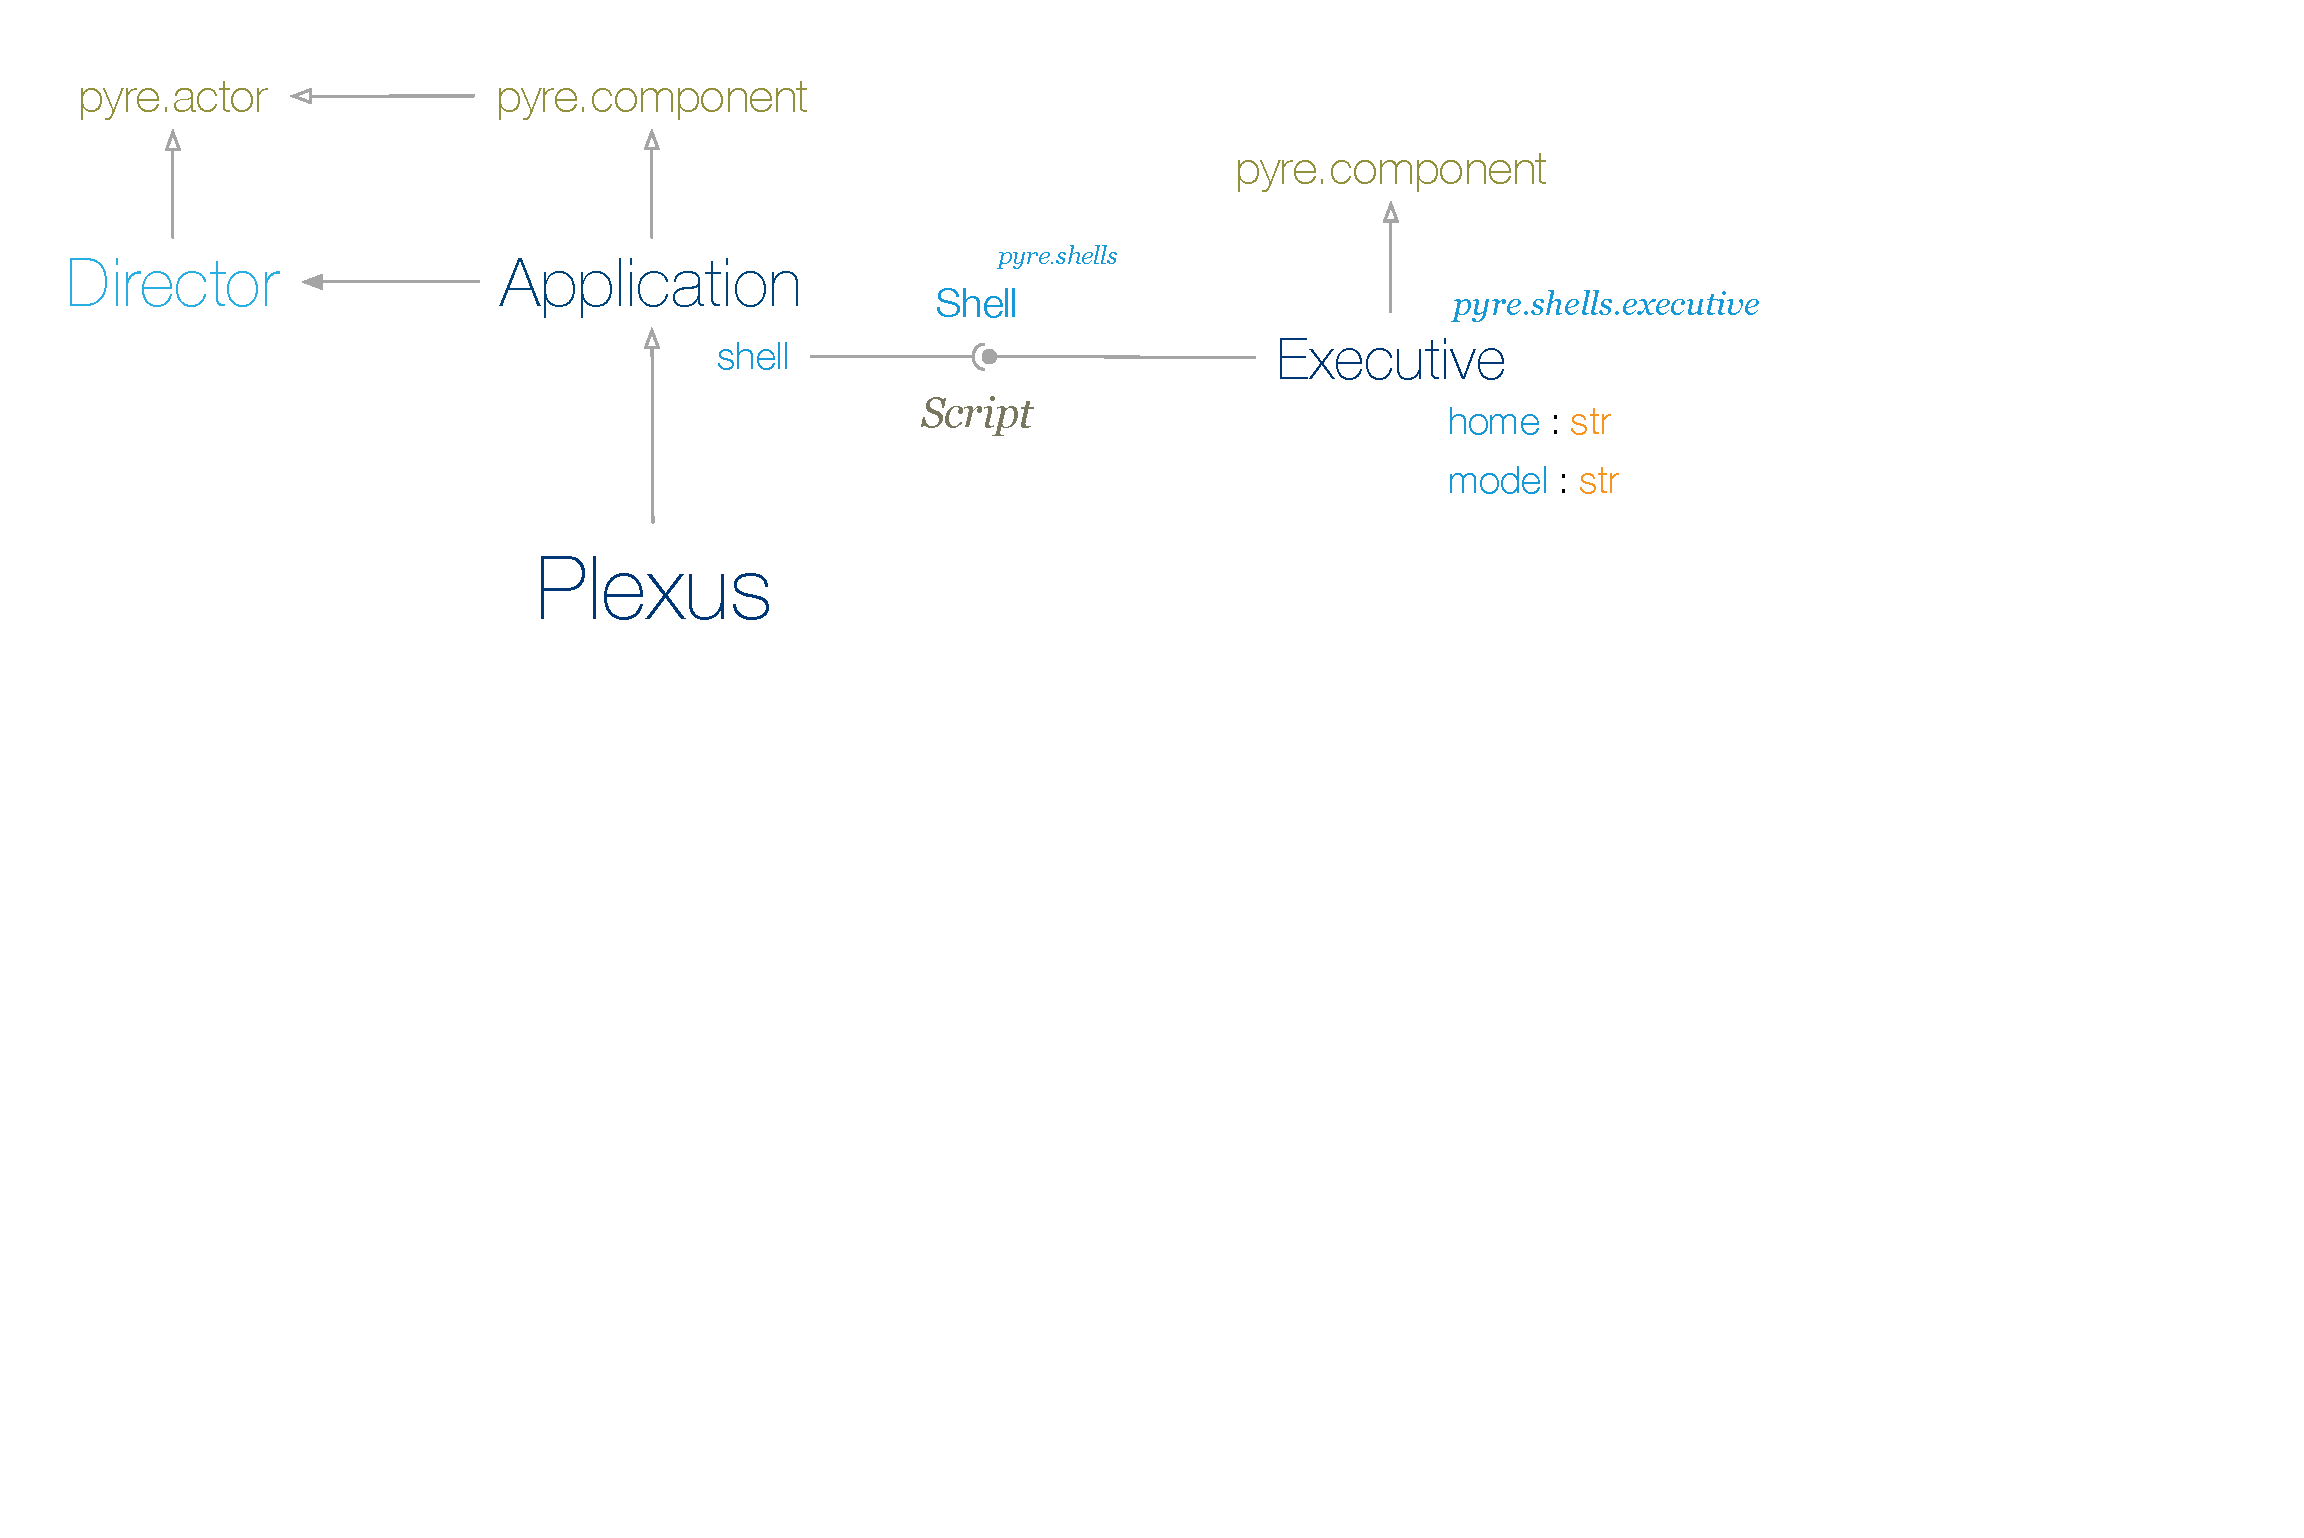
\includegraphics[height=0.9\textheight]{pyre-plexus-executive}}
  \only<5>{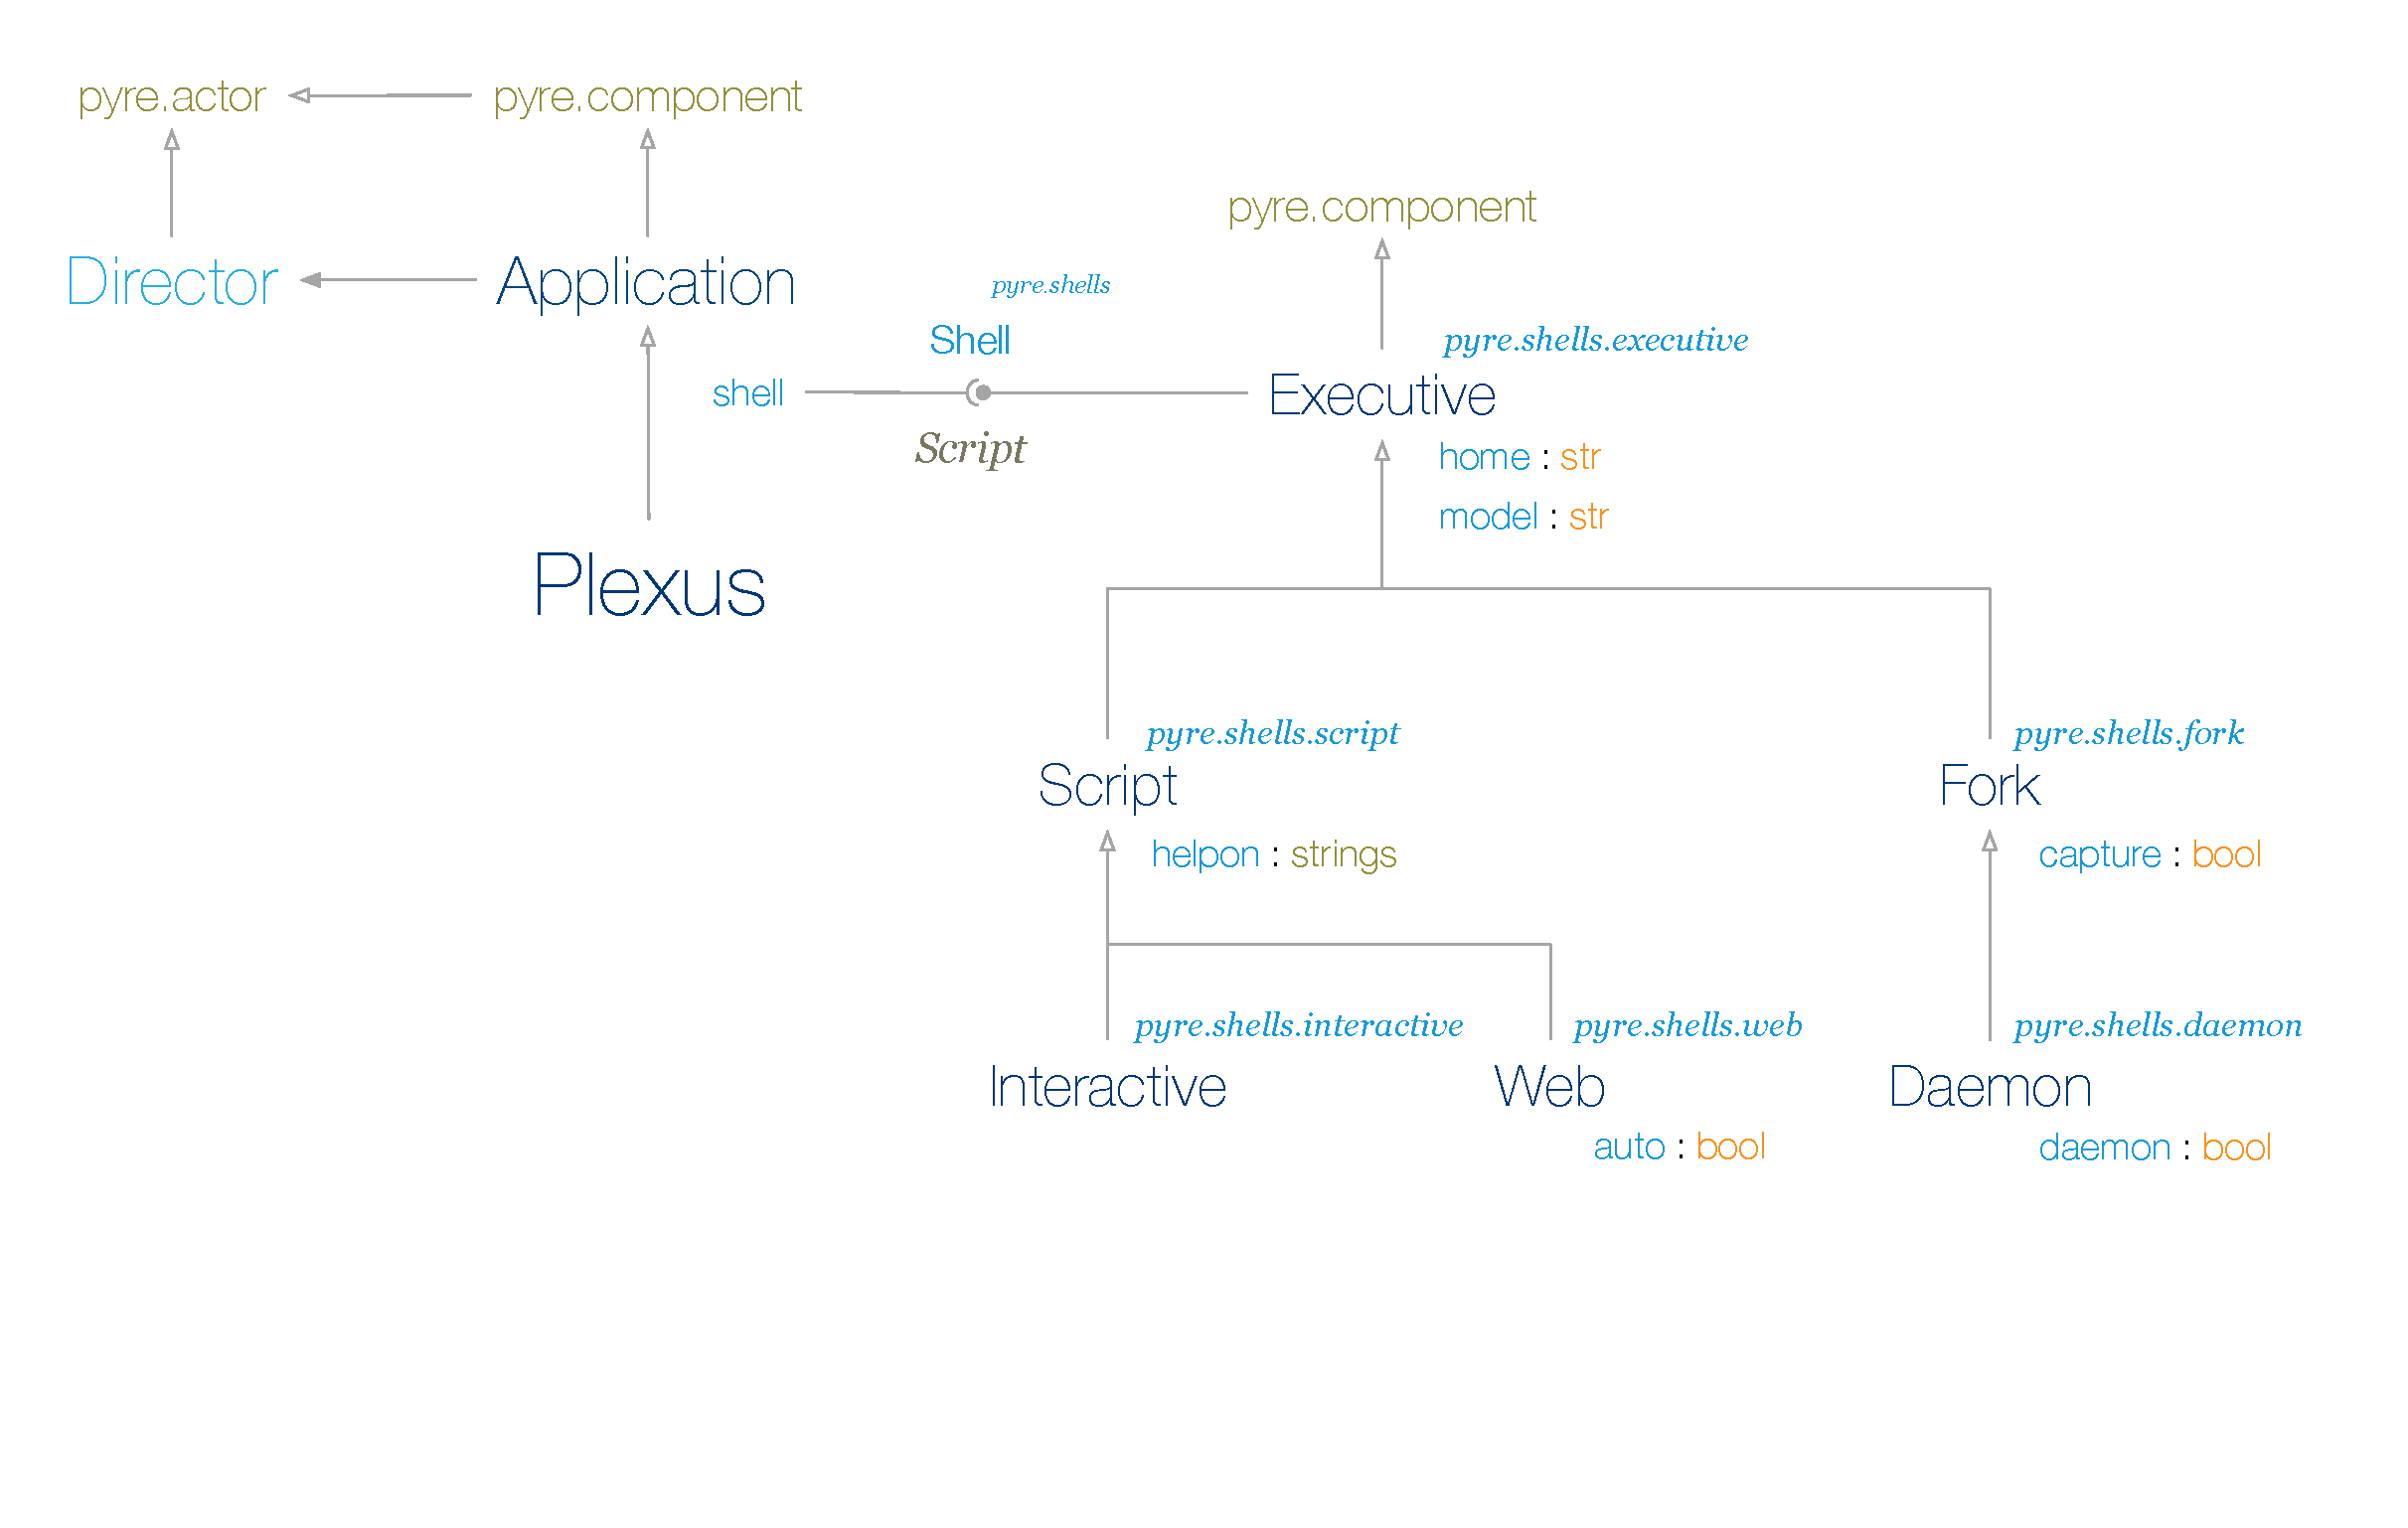
\includegraphics[height=0.9\textheight]{pyre-plexus-shells}}
  \only<6>{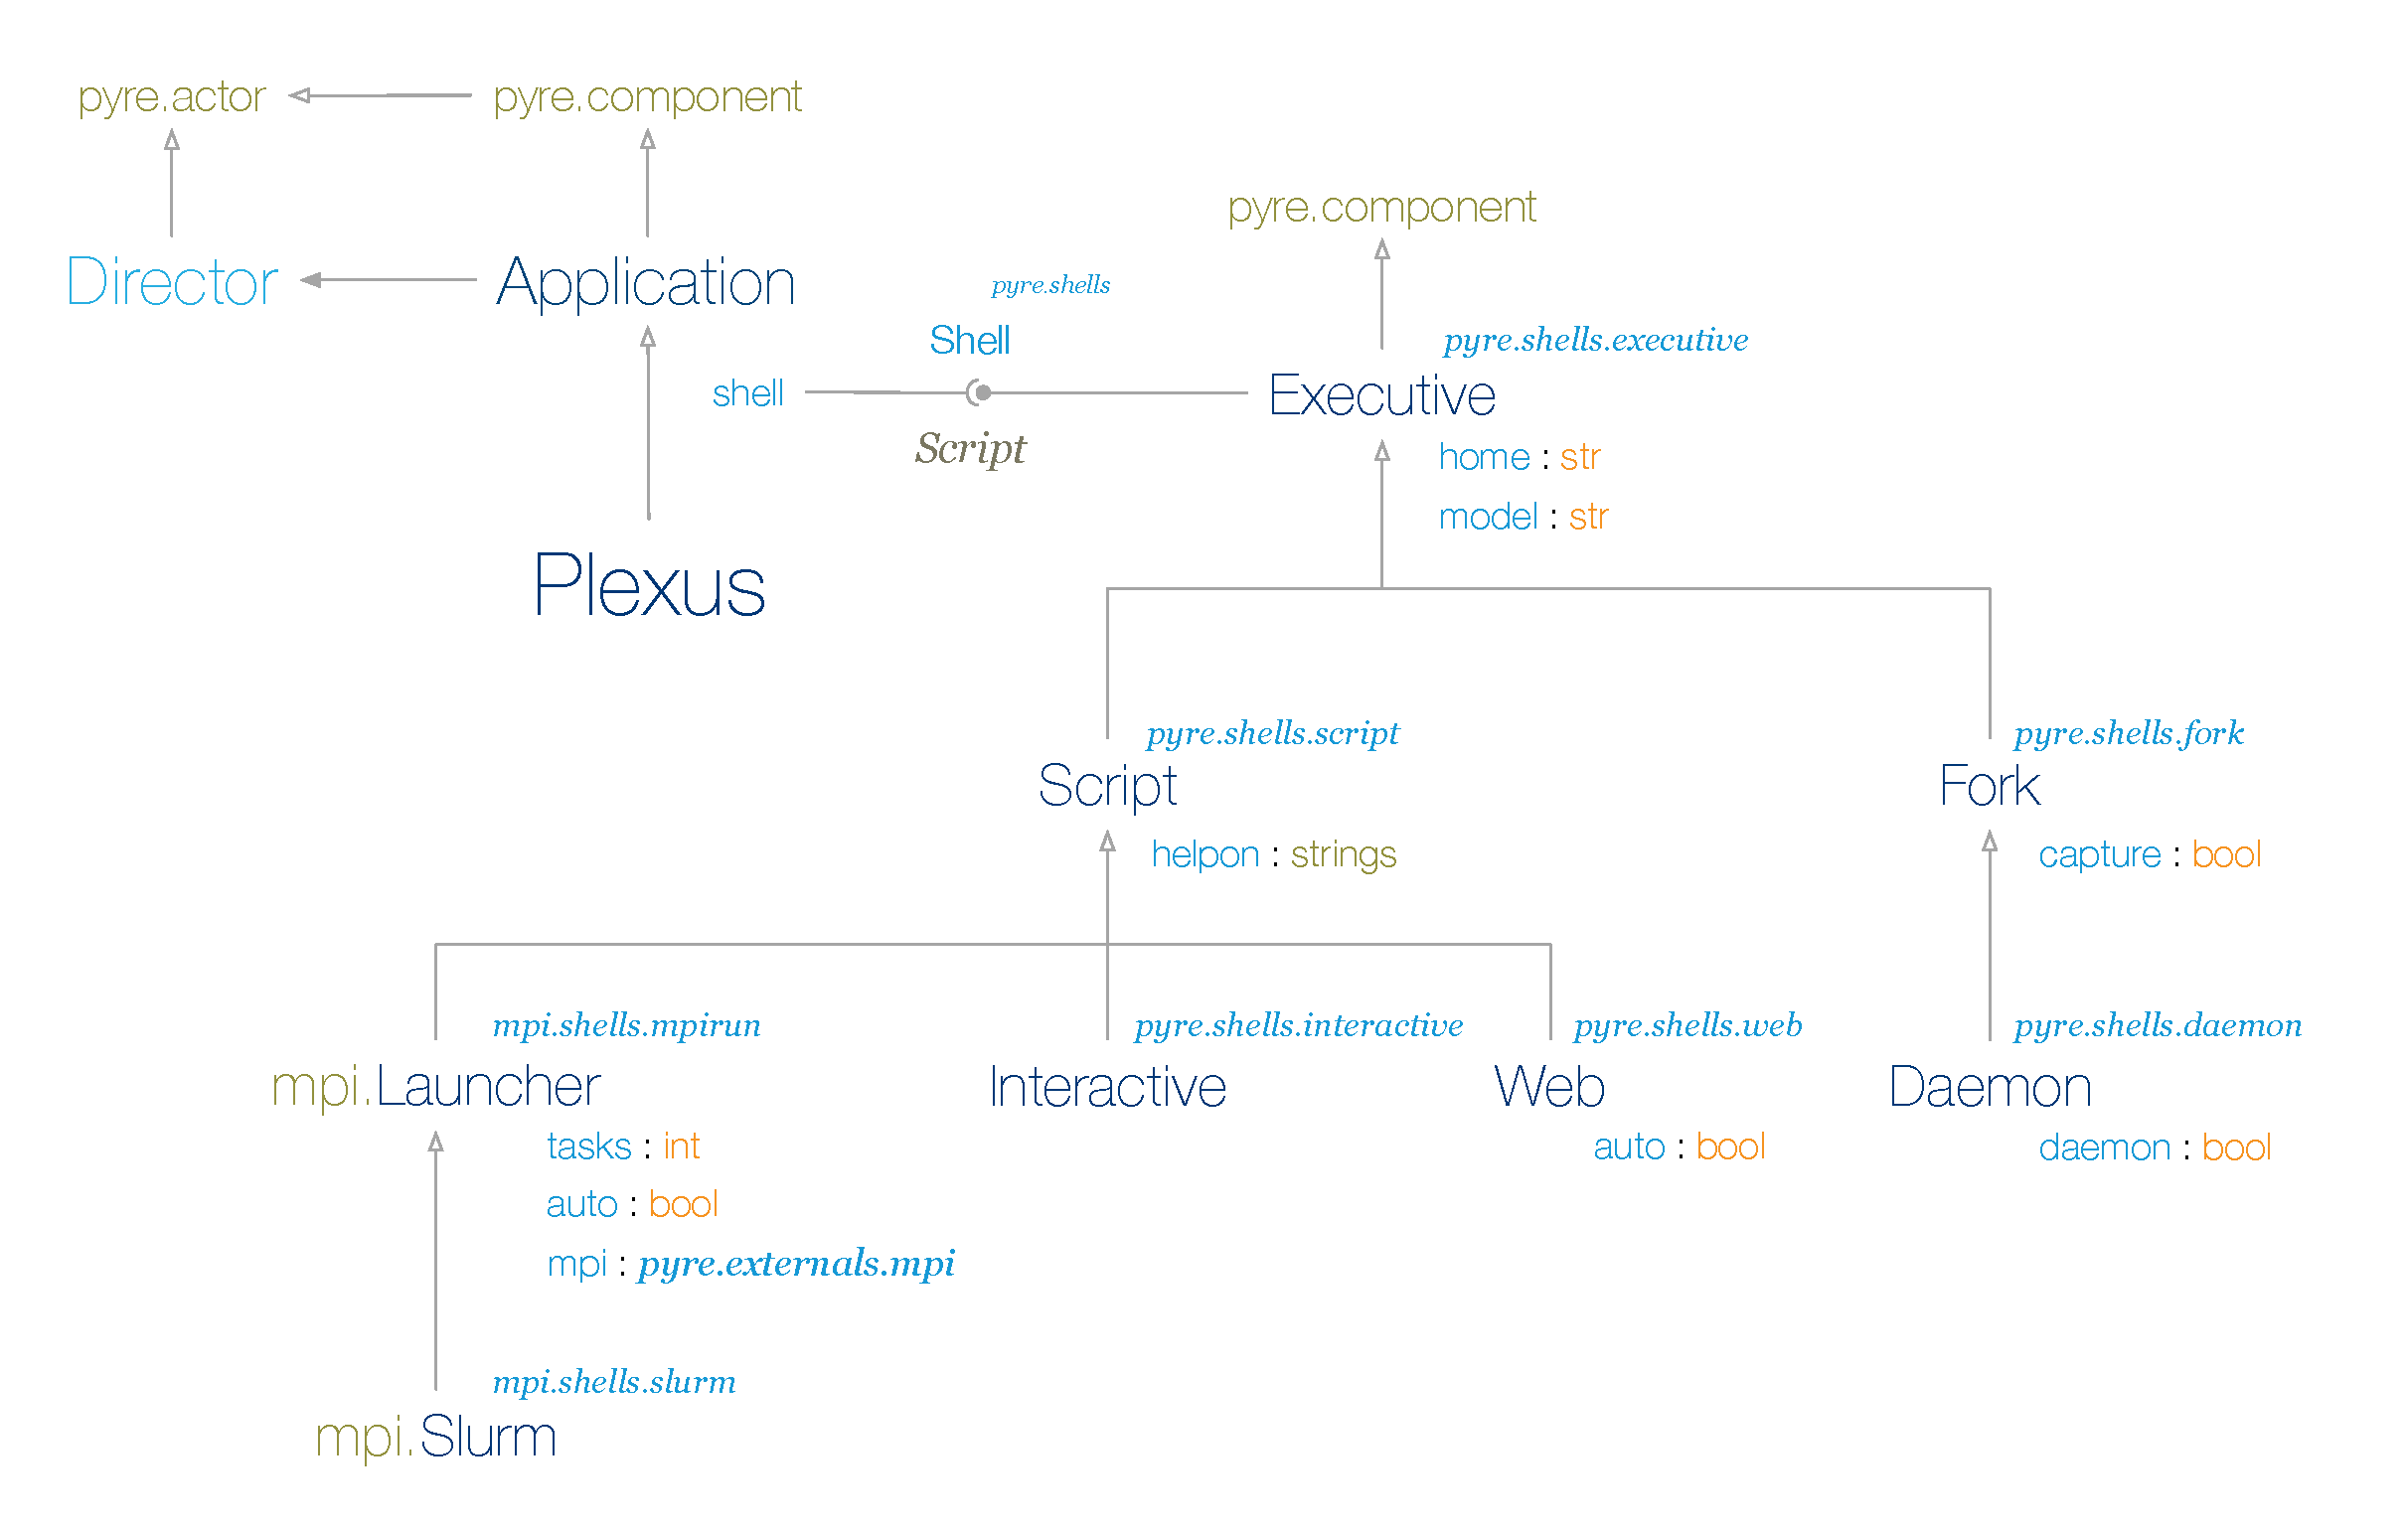
\includegraphics[height=0.9\textheight]{pyre-plexus-mpi}}
%
\end{frame}

% --------------------------------------

\TODO{
  \item show a trivial script
  \item show a simple application
  \item explain plexus
  \item convert simple app into a plexus action
  \item more on configuration files
  \item private filesystems
  \item the standard layout
}


%%% Local Variables:
%%% mode: latex
%%% TeX-master: "../pyre"
%%% End:

% end of file
